\chapter{प्रकाश-संश्लेषण और स्वपोषण}\label{ch:b1:photosynthesis}

खरगोश, बाँज, पाठक और इस पन्ने का हर ग्राम कार्बन कभी हवा की कार्बन
डाइऑक्साइड था, और उसे किसी \omterm{def:b1:flowering-plant-organization:organs}{पत्ती} ने --- या किसी शैवाल ने, या किसी
सायनोबैक्टीरियम ने --- सूर्य के प्रकाश की ऊर्जा से शर्करा में स्थिर किया
था। अभिक्रिया, यानी छह $\mathrm{CO_2}$ और छह जल से एक ग्लूकोज़ तथा छह
ऑक्सीजन, \qty{2870}{kJ/mol} की चढ़ाई है; और कोई \omterm{def:b1:flowering-plant-organization:organs}{पत्ती} उसे इस तरह चलाती
है कि प्रकाश से जल तोड़ती है, इलेक्ट्रॉन NADPH पर और ऊर्जा \omterm{def:b1:water-small-molecules:atp}{ATP} पर संचित
करती है, और दोनों को उस चक्र में ख़र्च करती है जो शर्करा बनाता है। यह
अध्याय \omterm{def:b1:photosynthesis:chloroplast}{हरितलवक} का, वर्णकों और उन प्रकाश अभिक्रियाओं का जो \omterm{def:b1:water-small-molecules:atp}{ATP} तथा NADPH
बनाती हैं, उस \omterm{def:b1:photosynthesis:fixation}{कैल्विन चक्र} का जो कार्बन स्थिर करता है, प्रकाश-श्वसन नाम
के रिसाव और उसे सील करने वाली दो अभिकल्पनाओं का, और सामान्य रूप से
\omterm{def:b1:photosynthesis:autotrophy}{स्वपोषण} क्या है इसका वर्णन करता है।

\section{हरितलवक और उसके वर्णक}

\begin{definition}[हरितलवक]\label{def:b1:photosynthesis:chloroplast}
\emph{हरितलवक}\index{हरितलवक} \qtyrange{3}{10}{\micro m} लंबा एक
लेंस-आकार का \omterm{def:b1:cell-unit-of-life:prokeuk}{कोशिकांग} है जिसकी सीमा दो आवरण झिल्लियाँ बनाती हैं; उसका
भीतरी भाग, यानी \emph{पीठिका}\index{पीठिका}, कार्बन-स्थिरीकरण के \omterm{def:b1:enzymes:enzyme}{एंजाइम},
मंड-कण, राइबोसोम और एक वर्तुल \omterm{def:b1:nucleic-acids:chain}{DNA} रखता है; और पीठिका के भीतर झिल्लियों का
एक तीसरा तंत्र, यानी \emph{थाइलेकॉइड}\index{थाइलेकॉइड}, चपटी थैलियाँ
बनाता है जो \emph{ग्रैना} में चिनी होती हैं और पटलिकाओं से जुड़ी, और जो
एक सतत \emph{थाइलेकॉइड अवकाशिका} घेरती हैं। \omterm{prop:b1:photosynthesis:lightreactions}{प्रकाश अभिक्रियाएँ}
थाइलेकॉइड झिल्ली में होती हैं; कार्बन-स्थिरीकरण पीठिका में। किसी
पर्ण-कोशिका में \qtyrange{20}{100}{} हरितलवक होते हैं; और \omterm{def:b1:flowering-plant-organization:organs}{पत्ती} के एक वर्ग
मिलीमीटर में पाँच लाख।
\end{definition}

\begin{omfigure}
\begin{tikzpicture}
  \node[anchor=south west, inner sep=0] (img) at (0,0)
    {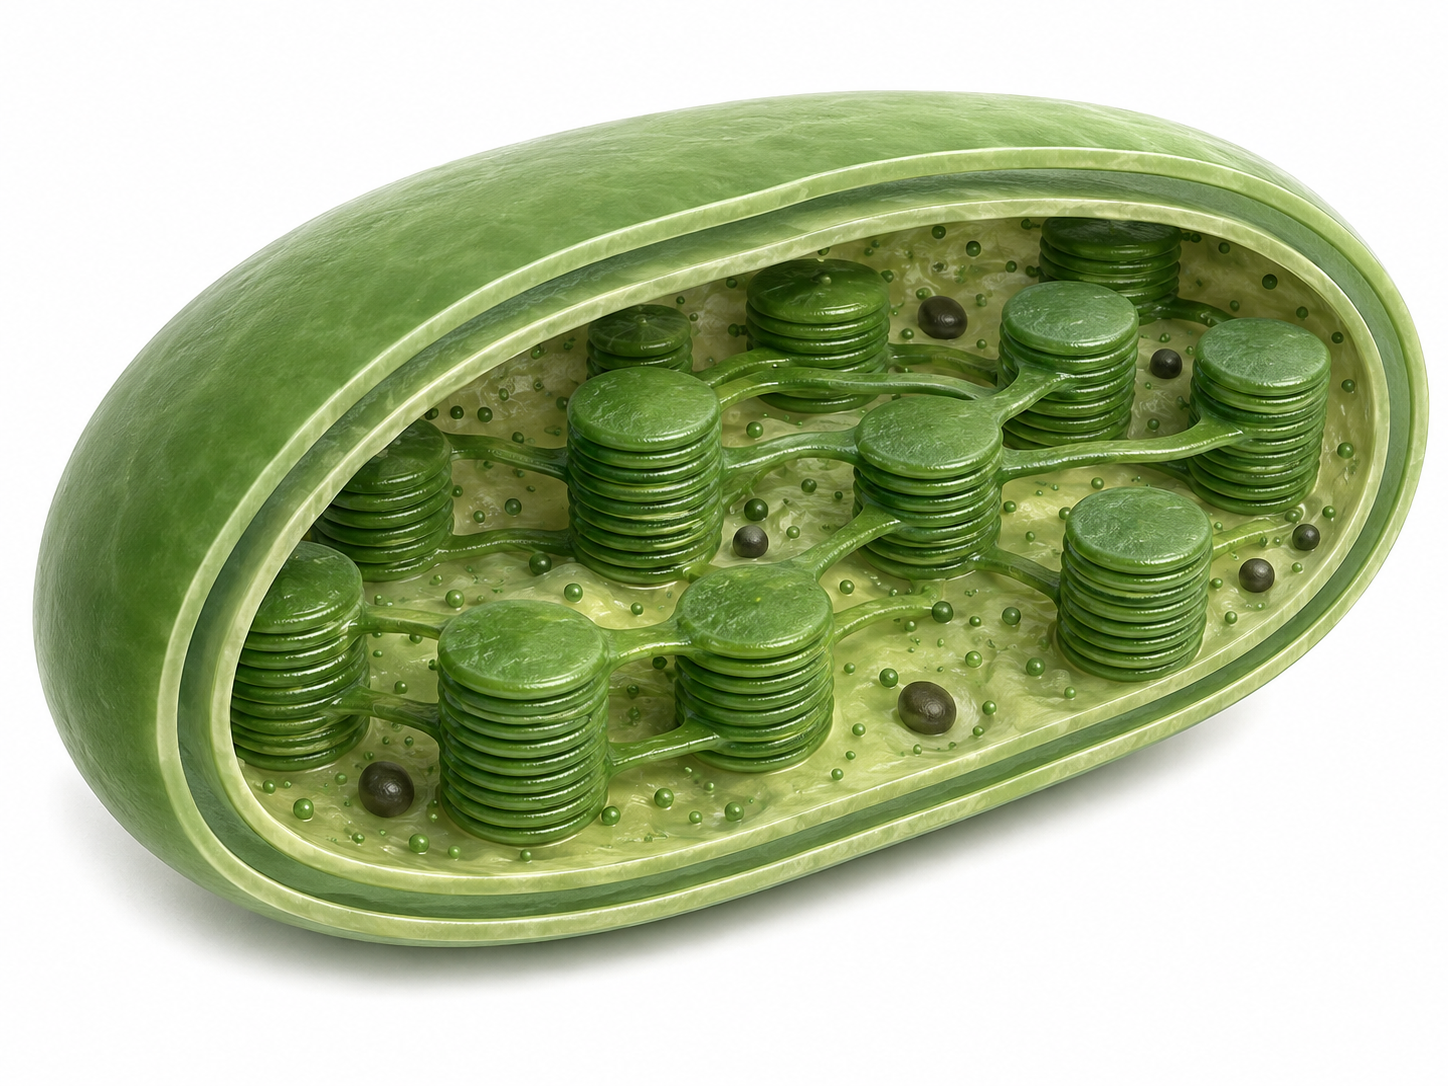
\includegraphics[width=0.56\linewidth]{images/book3/ai/fig-chloroplast-cutaway.png}};
  \begin{scope}[x={(img.south east)}, y={(img.north west)},
      every node/.style={font=\small}]
    \draw[omDef, thick] (0.12,0.50) -- (-0.03,0.66) node[left, align=right] {दो आवरण\\ झिल्लियाँ};
    \draw[omDef, thick] (0.48,0.60) -- (0.48,1.08) node[above] {ग्रैनम: थाइलेकॉइडों की एक चट्टी};
    \draw[omDef, thick] (0.62,0.52) -- (1.03,0.62) node[right] {पीठिका पटलिका};
    \draw[omDef, thick] (0.35,0.24) -- (-0.03,0.16) node[left] {पीठिका};
    \draw[omDef, thick] (0.86,0.50) -- (1.03,0.40) node[right] {मंड-कण};
  \end{scope}
\end{tikzpicture}

{\small खोलकर दिखाया गया एक \omterm{def:b1:photosynthesis:chloroplast}{हरितलवक}। \omterm{def:b1:photosynthesis:chloroplast}{पीठिका} के चारों ओर दो आवरण
झिल्लियाँ; भीतर, थाइलेकॉइडों की चट्टियाँ (ग्रैना) जो पटलिकाओं से जुड़ी हैं
और एक ही अवकाशिका घेरती हैं। प्रकाश \omterm{def:b1:photosynthesis:chloroplast}{थाइलेकॉइड} झिल्ली में पकड़ा जाता है
और शर्करा \omterm{def:b1:photosynthesis:chloroplast}{पीठिका} में बनती है।}
\end{omfigure}

\begin{definition}[प्रकाश-संश्लेषी वर्णक]\label{def:b1:photosynthesis:pigments}
\emph{पर्णहरित}\index{पर्णहरित} $a$ और $b$ किसी मैग्नीशियम परमाणु के
चारों ओर पॉर्फ़िरिन वलय हैं, जिनकी एक लंबी जलविरागी पूँछ उन्हें
\omterm{def:b1:photosynthesis:chloroplast}{थाइलेकॉइड} झिल्ली में टिकाए रखती है; वे नीला (\qtyrange{430}{450}{nm}) और
लाल (\qtyrange{640}{680}{nm}) प्रकाश अवशोषित करते हैं और हरा परावर्तित।
\emph{कैरोटिनॉइड}\index{कैरोटिनॉइड} (\omterm{def:b1:lipids:steroids}{आइसोप्रीनॉइड}, \cref{ch:b1:lipids})
नीला-हरा प्रकाश अवशोषित करते हैं और ऊर्जा पर्णहरित तक पहुँचाते हैं, तथा
अतिरिक्त उत्तेजन शमित करके उसकी रक्षा करते हैं। कुछ सौ वर्णक अणु,
\omterm{def:b1:proteins:peptide}{प्रोटीनों} पर किसी \emph{ऐंटेना} (प्रकाश-संचयी संकुल) के रूप में थमे हुए,
हर अवशोषित फ़ोटॉन की ऊर्जा पर्णहरित $a$ के एक विशेष युग्म तक कीप की तरह
पहुँचा देते हैं, यानी \emph{अभिक्रिया केंद्र} तक, जहाँ वह रसायन में बदल
जाती है।
\end{definition}

\begin{omfigure}
\begin{tikzpicture}
\begin{axis}[
  width=0.88\linewidth, height=6.2cm,
  axis x line=bottom, axis y line=left,
  xmin=400, xmax=720, ymin=0, ymax=1.1,
  xlabel={तरंगदैर्घ्य (\unit{nm})}, ylabel={अवशोषण, या दर (सापेक्ष)},
  xlabel style={font=\small, at={(axis description cs:0.5,-0.12)}, anchor=north},
  ylabel style={font=\small},
  tick label style={font=\small}, xtick={400,450,500,550,600,650,700}, ytick={0,0.5,1},
  legend style={font=\small, at={(0.5,0.98)}, anchor=north, draw=none},
  clip=false,
]
\addplot[very thick, omDef, domain=400:720, samples=160] {exp(-((x-430)/18)^2) + 0.85*exp(-((x-662)/14)^2) + 0.05};
\addlegendentry{पर्णहरित $a$ का अवशोषण}
\addplot[very thick, omExo, domain=400:720, samples=160] {0.7*exp(-((x-455)/20)^2) + 0.5*exp(-((x-645)/14)^2) + 0.05};
\addlegendentry{पर्णहरित $b$ का अवशोषण}
\addplot[very thick, omProp, domain=400:720, samples=160] {0.75*exp(-((x-470)/25)^2) + 0.05};
\addlegendentry{कैरोटिनॉइडों का अवशोषण}
\addplot[very thick, dashed, omThm, domain=400:720, samples=160] {0.9*exp(-((x-440)/30)^2) + 0.35*exp(-((x-520)/50)^2) + 0.85*exp(-((x-660)/22)^2) + 0.1};
\addlegendentry{क्रिया स्पेक्ट्रम: $\mathrm{O_2}$ मुक्ति की दर}
\end{axis}
\end{tikzpicture}

{\small तीनों वर्णक-वर्गों के अवशोषण स्पेक्ट्रम और प्रकाश-संश्लेषण का
क्रिया स्पेक्ट्रम (यानी हर तरंगदैर्घ्य पर ऑक्सीजन मुक्ति की दर)। क्रिया
स्पेक्ट्रम \omterm{def:b1:photosynthesis:pigments}{पर्णहरितों} के पीछे चलता है, और नीले-हरे में उसे \omterm{def:b1:photosynthesis:pigments}{कैरोटिनॉइड} भर
देते हैं: जो भी वर्णक अवशोषित करता है वह योगदान देता है।}
\end{omfigure}

\begin{proposition}[क्रिया स्पेक्ट्रम वर्णकों के पीछे चलता है]\label{prop:b1:photosynthesis:engelmann}
प्रकाश-संश्लेषण को वही प्रकाश चलाता है जिसे वर्णक अवशोषित करते हैं: वह लाल
और नीले प्रकाश में सबसे तेज़ है, और हरे में सबसे धीमा।
\end{proposition}
\begin{proof}[साक्ष्य]
एंगेलमान (1882) ने अपने सूक्ष्मदर्शी के नीचे प्रक्षेपित किसी स्पेक्ट्रम
के आरपार किसी शैवाल का तंतु रखा और ऑक्सीजन खोजते जीवाणु मिलाए: वे वहीं
इकट्ठे हुए जहाँ लाल और नीला प्रकाश पड़ रहा था, हरे में नहीं (जो लाइसेयी
खंड से याद है)। किसी ऑक्सीजन इलेक्ट्रोड से मापने पर हर तरंगदैर्घ्य की दर
ऊपर वाला क्रिया स्पेक्ट्रम देती है, जो \omterm{def:b1:photosynthesis:pigments}{पर्णहरितों} के अवशोषण के पीछे चलता
है; और नीले-हरे में जो अधिकता है वह \omterm{def:b1:photosynthesis:pigments}{कैरोटिनॉइडों} का योगदान है, जो दिखाता
है कि वे अपनी ऊर्जा आगे पहुँचाते हैं।
\end{proof}

\section{प्रकाश अभिक्रियाएँ}

\begin{proposition}[प्रकाश अभिक्रियाएँ क्या करती हैं]\label{prop:b1:photosynthesis:lightreactions}
\index{प्रकाश अभिक्रियाएँ}
\omterm{def:b1:photosynthesis:chloroplast}{थाइलेकॉइड} झिल्ली में प्रकाश की ऊर्जा से इलेक्ट्रॉन जल से
$\mathrm{NADP^+}$ तक ले जाए जाते हैं --- चढ़ाई पर, \qty{1.1}{V} के किसी
अपचयोपचय विभवांतर के विरुद्ध --- और अवकाशिका में प्रोटॉन पंप किए जाते हैं:
\[
2\,\mathrm{H_2O} + 2\,\mathrm{NADP^+} + 3\,\mathrm{ADP} + 3\,\mathrm{P_i}
\xrightarrow{\ 8\ \text{फ़ोटॉन}\ }
\mathrm{O_2} + 2\,\mathrm{NADPH} + 2\,\mathrm{H^+} + 3\,\mathrm{ATP} .
\]
जो ऑक्सीजन छूटती है वह जल की ऑक्सीजन है, कार्बन डाइऑक्साइड की नहीं;
NADPH अपचायक शक्ति ढोता है और \omterm{def:b1:water-small-molecules:atp}{ATP} वह ऊर्जा जिसे \omterm{def:b1:photosynthesis:fixation}{कैल्विन चक्र} ख़र्च
करेगा।
\end{proposition}
\begin{proof}[साक्ष्य]
हिल (1937) ने दिखाया कि प्रकाश में अलग किए गए \omterm{def:b1:photosynthesis:chloroplast}{हरितलवक} $\mathrm{CO_2}$ के
बिना भी ऑक्सीजन छोड़ते हैं यदि कोई कृत्रिम इलेक्ट्रॉन ग्राही उपस्थित हो:
यानी जल का टूटना कार्बन-स्थिरीकरण से अलग किया जा सकता है।
रूबेन और केमन (1941) ने शैवालों को भारी ऑक्सीजन से चिह्नित जल खिलाया और
चिह्न छूटी हुई $\mathrm{O_2}$ में पाया, और तब नहीं जब चिह्न
$\mathrm{CO_2}$ में था। एमरसन (1957) ने पाया कि \qty{700}{nm} का लाल
प्रकाश, जो अकेले लगभग बेकार है, और \qty{680}{nm} का प्रकाश
मिलकर उनकी अलग-अलग दरों के योग से अधिक देते हैं: यानी अलग-अलग वर्णकों वाले
दो प्रकाशतंत्रों को शृंखला में काम करना चाहिए।
\end{proof}

\begin{definition}[प्रकाशतंत्र और Z-योजना]\label{def:b1:photosynthesis:zscheme}
\index{प्रकाशतंत्र}\index{Z-योजना}
\omterm{def:b1:photosynthesis:chloroplast}{थाइलेकॉइड} झिल्ली में दो \emph{प्रकाशतंत्र} बैठे हैं।
\emph{प्रकाशतंत्र II} (PSII, अभिक्रिया केंद्र P680) में कोई अवशोषित
फ़ोटॉन उस विशेष युग्म के एक इलेक्ट्रॉन को ऊँची ऊर्जा तक उठा देता है;
इलेक्ट्रॉन निकल जाता है, और ऑक्सीकृत P680, जो सबसे प्रबल जैविक ऑक्सीकारक
है, जल से एक इलेक्ट्रॉन ले लेता है: कोई मैंगनीज़ गुच्छ दो जल-अणुओं को
$\mathrm{O_2}$, चार प्रोटॉन (जो अवकाशिका में छोड़े जाते हैं)
और चार इलेक्ट्रॉनों में तोड़ता है, एक बार में एक फ़ोटॉन। इलेक्ट्रॉन किसी
\emph{इलेक्ट्रॉन-अभिगमन शृंखला} से नीचे उतरता है --- प्लास्टोक्विनोन,
\emph{साइटोक्रोम $b_6f$ संकुल}, प्लास्टोसायनिन --- और जो ऊर्जा वह खोता है
वह अवकाशिका में प्रोटॉन पंप करती है। \emph{प्रकाशतंत्र I} (PSI,
P700) में एक दूसरा फ़ोटॉन उसे फिर उठा देता है, इतने नीचे विभव तक कि वह
फ़ेरेडॉक्सिन को और फिर $\mathrm{NADP^+}$ को NADPH में अपचयित कर सके।
अपचयोपचय विभव के पैमाने पर बनाएँ तो यह पथ एक Z है: प्रकाश से दो चढ़ाइयाँ,
रसायन से दो उतराइयाँ।
\end{definition}

\begin{omfigure}
\begin{tikzpicture}[font=\footnotesize, >=Stealth, line cap=round,
  st/.style={draw, thick, rounded corners=2pt, inner sep=2pt}]
  % redox potential axis (vertical, more negative up)
  \draw[->, thick] (0,0) -- (0,6.4) node[above, font=\small] {अपचयोपचय विभव $E'_0$ (V)};
  \foreach \y/\l in {0.4/{$+1.0$}, 1.9/{$+0.5$}, 3.4/{$0$}, 4.9/{$-0.5$}, 6.0/{$-0.9$}} { \draw (-0.1,\y) -- (0.1,\y) node[left, xshift=-4pt] {\l}; }
  % PSII
  \node[st, fill=omDef!15] (h2o) at (1.7,1.0) {$\mathrm{H_2O}$};
  \node[st, fill=omDef!25] (p680) at (2.9,0.35) {P680};
  \node[st, fill=omDef!25] (p680s) at (2.9,5.7) {P680*};
  \draw[->, thick] (h2o) -- (p680);
  \node[anchor=west, font=\scriptsize] at (3.5,0.35) {$\to \mathrm{O_2} + 4\,\mathrm{H^+}$ अवकाशिका में};
  \draw[->, very thick, omProp] (p680) -- (p680s) node[pos=0.45, right, align=left] {फ़ोटॉन\\ (\qty{680}{nm})};
  % chain
  \node[st, fill=omThm!15] (pq) at (4.2,4.4) {PQ};
  \node[st, fill=omThm!15] (b6f) at (5.4,3.6) {cyt $b_6f$};
  \node[st, fill=omThm!15] (pc) at (6.5,2.8) {PC};
  \draw[->, thick] (p680s) -- (pq); \draw[->, thick] (pq) -- (b6f); \draw[->, thick] (b6f) -- (pc);
  \node[anchor=south west, align=left, font=\scriptsize, omThm] at (4.75,4.15) {$\mathrm{H^+}$ अवकाशिका में\\ पंप किए गए};
  % PSI
  \node[st, fill=omExo!25] (p700) at (7.7,2.3) {P700};
  \node[st, fill=omExo!25] (p700s) at (7.7,6.0) {P700*};
  \draw[->, thick] (pc) -- (p700);
  \draw[->, very thick, omProp] (p700) -- (p700s) node[pos=0.45, right, align=left] {फ़ोटॉन\\ (\qty{700}{nm})};
  \node[st, fill=omThm!15] (fd) at (9.1,5.2) {Fd};
  \node[st, fill=omExo!15] (nadp) at (10.5,4.6) {NADPH};
  \draw[->, thick] (p700s) -- (fd); \draw[->, thick] (fd) -- (nadp);
  \node[anchor=north, font=\scriptsize] at (10.5,4.3) {$E'_0 = \qty{-0.32}{V}$};
  % cyclic flow
  \draw[->, thick, dashed, gray] (fd) .. controls (7.2,5.5) and (4.4,5.5) .. (pq.north);
  \node[gray, font=\scriptsize, anchor=south] at (5.6,5.45) {चक्रीय प्रवाह (केवल ATP)};
\end{tikzpicture}

{\small \omterm{def:b1:photosynthesis:zscheme}{Z-योजना}। P680 द्वारा जल से लिए गए इलेक्ट्रॉन किसी फ़ोटॉन से उठाए
जाते हैं, उस शृंखला से उतरते हैं जो प्रोटॉन पंप करती है, P700 से फिर उठाए
जाते हैं और NADPH पर समाप्त होते हैं। ऊर्ध्व अक्ष अपचयोपचय विभव है, ऊपर
की ओर अधिक ऋणात्मक: चढ़ाई प्रकाश करता है, उतराई रसायन।}
\end{omfigure}

\begin{theorem}[ATP का रसोपरासरणी संश्लेषण]\label{thm:b1:photosynthesis:chemiosmosis}
\index{रसोपरासरण}\index{ATP सिंथेज़}
जल के टूटने से छूटे और साइटोक्रोम $b_6f$ संकुल से पंप किए गए प्रोटॉन
\omterm{def:b1:photosynthesis:chloroplast}{थाइलेकॉइड} अवकाशिका में जमा होते हैं, जो प्रकाश में गिरकर pH 5 हो जाती है
जबकि \omterm{def:b1:photosynthesis:chloroplast}{पीठिका} बढ़कर pH 8: यानी तीन मात्रकों का अंतर, लगभग \qty{0.18}{V} का
प्रोटॉन-प्रेरक बल, जो प्रति मोल प्रोटॉन \qty{17}{kJ} के बराबर है।
\emph{\omterm{thm:b1:photosynthesis:chemiosmosis}{ATP सिंथेज़}}, जो \omterm{def:b1:photosynthesis:chloroplast}{थाइलेकॉइड} झिल्ली पार करता एक घूर्णी प्रेरक है,
प्रोटॉनों को \omterm{def:b1:photosynthesis:chloroplast}{पीठिका} में वापस बहने देता है और उस ऊर्जा से ADP का
फ़ॉस्फ़ोरिलीकरण करता है: प्रति \omterm{def:b1:water-small-molecules:atp}{ATP} लगभग \qty{4}{H^+}। इलेक्ट्रॉन अभिगमन
और \omterm{def:b1:water-small-molecules:atp}{ATP} संश्लेषण केवल इसी प्रवणता से युग्मित हैं (मिचेल का रसोपरासरण
सिद्धांत, 1961)।
\end{theorem}
\begin{proof}[साक्ष्य]
यागेनडॉर्फ़ (1966) ने थाइलेकॉइडों को अँधेरे में किसी अम्ल-स्नान (pH 4) में
तब तक भिगोया जब तक उनकी अवकाशिका अम्लीय न हो गई, फिर उन्हें ADP और
फ़ॉस्फ़ेट के साथ अचानक pH 8 पर पहुँचा दिया: \omterm{def:b1:water-small-molecules:atp}{ATP} अँधेरे में ही बन गया, केवल
प्रवणता से। अयुग्मक --- यानी वे लिपिड-घुलनशील दुर्बल अम्ल जो झिल्लियों के
आरपार प्रोटॉन ढोते हैं --- \omterm{def:b1:water-small-molecules:atp}{ATP} संश्लेषण मिटा देते हैं जबकि इलेक्ट्रॉन
अभिगमन और ऑक्सीजन मुक्ति चलती रहती हैं, बल्कि तेज़ भी हो जाती हैं। अलग
किया गया \omterm{thm:b1:photosynthesis:chemiosmosis}{ATP सिंथेज़}, कृत्रिम पुटिकाओं में फिर बिठाने पर, कोई pH प्रवणता
थोपे जाने पर \omterm{def:b1:water-small-molecules:atp}{ATP} बनाता है, और न थोपे जाने पर \omterm{def:b1:water-small-molecules:atp}{ATP} का \omterm{prop:b1:water-small-molecules:families}{जल-अपघटन} करके प्रोटॉन
पंप करता है। तब से उस \omterm{def:b1:enzymes:enzyme}{एंजाइम} का घूमना सूक्ष्मदर्शी के नीचे, एक बार में एक
अणु, सीधे देखा जा चुका है।
\end{proof}

\begin{example}[चक्रीय और अचक्रीय प्रवाह]\label{ex:b1:photosynthesis:cyclic}
जल से NADPH तक का रैखिक पथ प्रति $\mathrm{O_2}$ दो
NADPH और लगभग तीन \omterm{def:b1:water-small-molecules:atp}{ATP} देता है; \omterm{def:b1:photosynthesis:fixation}{कैल्विन चक्र} को ठीक तीन \omterm{def:b1:water-small-molecules:atp}{ATP} से दो NADPH
का अनुपात चाहिए, और \omterm{def:b1:photosynthesis:chloroplast}{हरितलवक} के दूसरे कामों को और \omterm{def:b1:water-small-molecules:atp}{ATP} चाहिए।
जब \omterm{def:b1:water-small-molecules:atp}{ATP} कम पड़ता है, तब फ़ेरेडॉक्सिन के इलेक्ट्रॉन $\mathrm{NADP^+}$ पर
जाने के बजाय प्लास्टोक्विनोन पर लौट आते हैं (\emph{चक्रीय
प्रकाशफ़ॉस्फ़ोरिलीकरण}): अकेला PSI, प्रोटॉन पंप करता और \omterm{def:b1:water-small-molecules:atp}{ATP} बनाता,
बिना ऑक्सीजन या NADPH के। दोनों ढंग माँग के अनुसार संतुलित रहते हैं।
\end{example}

\section{कैल्विन चक्र}

\begin{definition}[कार्बन स्थिरीकरण]\label{def:b1:photosynthesis:fixation}
\index{कैल्विन चक्र}\index{RuBisCO}
\omterm{def:b1:photosynthesis:chloroplast}{पीठिका} का \emph{कैल्विन चक्र} $\mathrm{CO_2}$ को तीन चरणों में शर्करा
में स्थिर करता है। \emph{स्थिरीकरण}: \emph{RuBisCO} (राइबुलोस
बिसफ़ॉस्फ़ेट कार्बोक्सिलेज़/ऑक्सीजनेज़) $\mathrm{CO_2}$ को
राइबुलोस-1,5-बिसफ़ॉस्फ़ेट (RuBP, पाँच कार्बन) से जोड़ता है, और छह-कार्बन
वाला उत्पाद तुरंत 3-फ़ॉस्फ़ोग्लिसरेट के दो अणुओं
(3-PGA, तीन कार्बन) में टूट जाता है। \emph{अपचयन}: हर 3-PGA का \omterm{def:b1:water-small-molecules:atp}{ATP} से
फ़ॉस्फ़ोरिलीकरण होता है और NADPH से अपचयन, जिससे
ग्लिसरैल्डिहाइड-3-फ़ॉस्फ़ेट (G3P), यानी पहली शर्करा बनती है।
\emph{पुनर्जनन}: हर छह में से पाँच G3P, \omterm{def:b1:water-small-molecules:atp}{ATP} की क़ीमत पर, फिर से तीन RuBP
में सजा दिए जाते हैं, और एक G3P शुद्ध उत्पाद के रूप में चक्र से निकल जाता
है। एक G3P (तीन कार्बन) के लिए रससमीकरणमिति यह है
\[
3\,\mathrm{CO_2} + 9\,\mathrm{ATP} + 6\,\mathrm{NADPH} + 6\,\mathrm{H^+}
\to \text{G3P} + 9\,\mathrm{ADP} + 8\,\mathrm{P_i} + 6\,\mathrm{NADP^+} ;
\]
दो G3P एक ग्लूकोज़ बनाते हैं: प्रति ग्लूकोज़ \qty{18}{} \omterm{def:b1:water-small-molecules:atp}{ATP} और \qty{12}{NADPH}।
\end{definition}

\begin{omfigure}
\begin{tikzpicture}[font=\footnotesize, >=Stealth, line cap=round,
  box/.style={draw, thick, rounded corners=3pt, minimum height=8mm, align=center, fill=white}]
  \node[box, fill=omDef!15] (rubp) at (0,2.6) {3 RuBP\\ ($3\times$ C5)};
  \node[box, fill=omDef!15] (pga) at (5.0,2.6) {6 3-PGA\\ ($6\times$ C3)};
  \node[box, fill=omDef!15] (g3p) at (5.0,-0.4) {6 G3P\\ ($6\times$ C3)};
  \node[box, fill=omExo!20] (out) at (9.2,-0.4) {1 G3P बाहर\\ (शुद्ध लाभ: 3 C)};
  \draw[->, very thick, omThm] (rubp) -- (pga) node[midway, above, align=center] {स्थिरीकरण (RuBisCO)\\ $+\,3\,\mathrm{CO_2}$};
  \draw[->, very thick, omThm] (pga) -- (g3p) node[midway, right, align=left] {अपचयन\\ $6\,\mathrm{ATP}$, $6\,\mathrm{NADPH}$};
  \draw[->, very thick, omThm] (g3p) -- (out);
  \draw[->, very thick, omThm] (g3p) -| (rubp);
  \node[anchor=north, align=center, omThm] at (2.4,-0.95) {पुनर्जनन: 5 G3P $\to$ 3 RuBP\\ $3\,\mathrm{ATP}$};
  \node[anchor=north, align=center, gray] at (4.6,-1.7) {प्रति फेरा (तीन $\mathrm{CO_2}$): 9 ATP, 6 NADPH, एक G3P कमाया\\ दो फेरे: एक ग्लूकोज़, 18 ATP, 12 NADPH};
\end{tikzpicture}

{\small $\mathrm{CO_2}$ के तीन अणुओं के लिए \omterm{def:b1:photosynthesis:fixation}{कैल्विन चक्र}: तीन
RuBP छह 3-PGA में स्थिर, छह G3P में अपचयित, जिनमें से एक निकल जाता है और
पाँच तीनों RuBP का पुनर्जनन करते हैं। कार्बन हर चरण पर संरक्षित है
($15 + 3 = 18 = 3 + 15$)।}
\end{omfigure}

\begin{proposition}[कैल्विन का साक्ष्य]\label{prop:b1:photosynthesis:calvin}
$\mathrm{CO_2}$ स्थिरीकरण का पहला स्थायी उत्पाद 3-फ़ॉस्फ़ोग्लिसरेट है,
और ग्राही राइबुलोस बिसफ़ॉस्फ़ेट।
\end{proposition}
\begin{proof}[साक्ष्य]
कैल्विन और बेन्सन (1948--1954) ने शैवालों को किसी चपटे फ़्लास्क
(``लॉलीपॉप'') में प्रकाशित किया, $\mathrm{^{14}CO_2}$ भीतर डाला, और
सेकंडों बाद नमूनों को उबलते ऐल्कोहॉल में मार डाला; और द्विविमीय काग़ज़
वर्णलेखन तथा स्वप्रकाशचित्रिकी ने दिखाया कि चिह्न कहाँ है। पाँच सेकंड बाद
वह लगभग पूरा 3-PGA में था; और लंबे समय तक रखने पर वह शर्करा फ़ॉस्फ़ेटों
में और फिर सुक्रोस तथा \omterm{def:b1:carbohydrates:polysaccharide}{मंड} में फैल गया। जब
$\mathrm{CO_2}$ अचानक हटा दी गई तो RuBP जमा हुआ और 3-PGA गिरा;
और जब प्रकाश बंद कर दिया गया तो 3-PGA जमा हुआ और RuBP गिरा --- इसलिए
RuBP वह ग्राही है जिसे स्थिरीकरण खपाता है, और 3-PGA वह उत्पाद जिसे प्रकाश
के \omterm{def:b1:water-small-molecules:atp}{ATP} तथा NADPH खपाते हैं।
\end{proof}

\begin{omfigure}
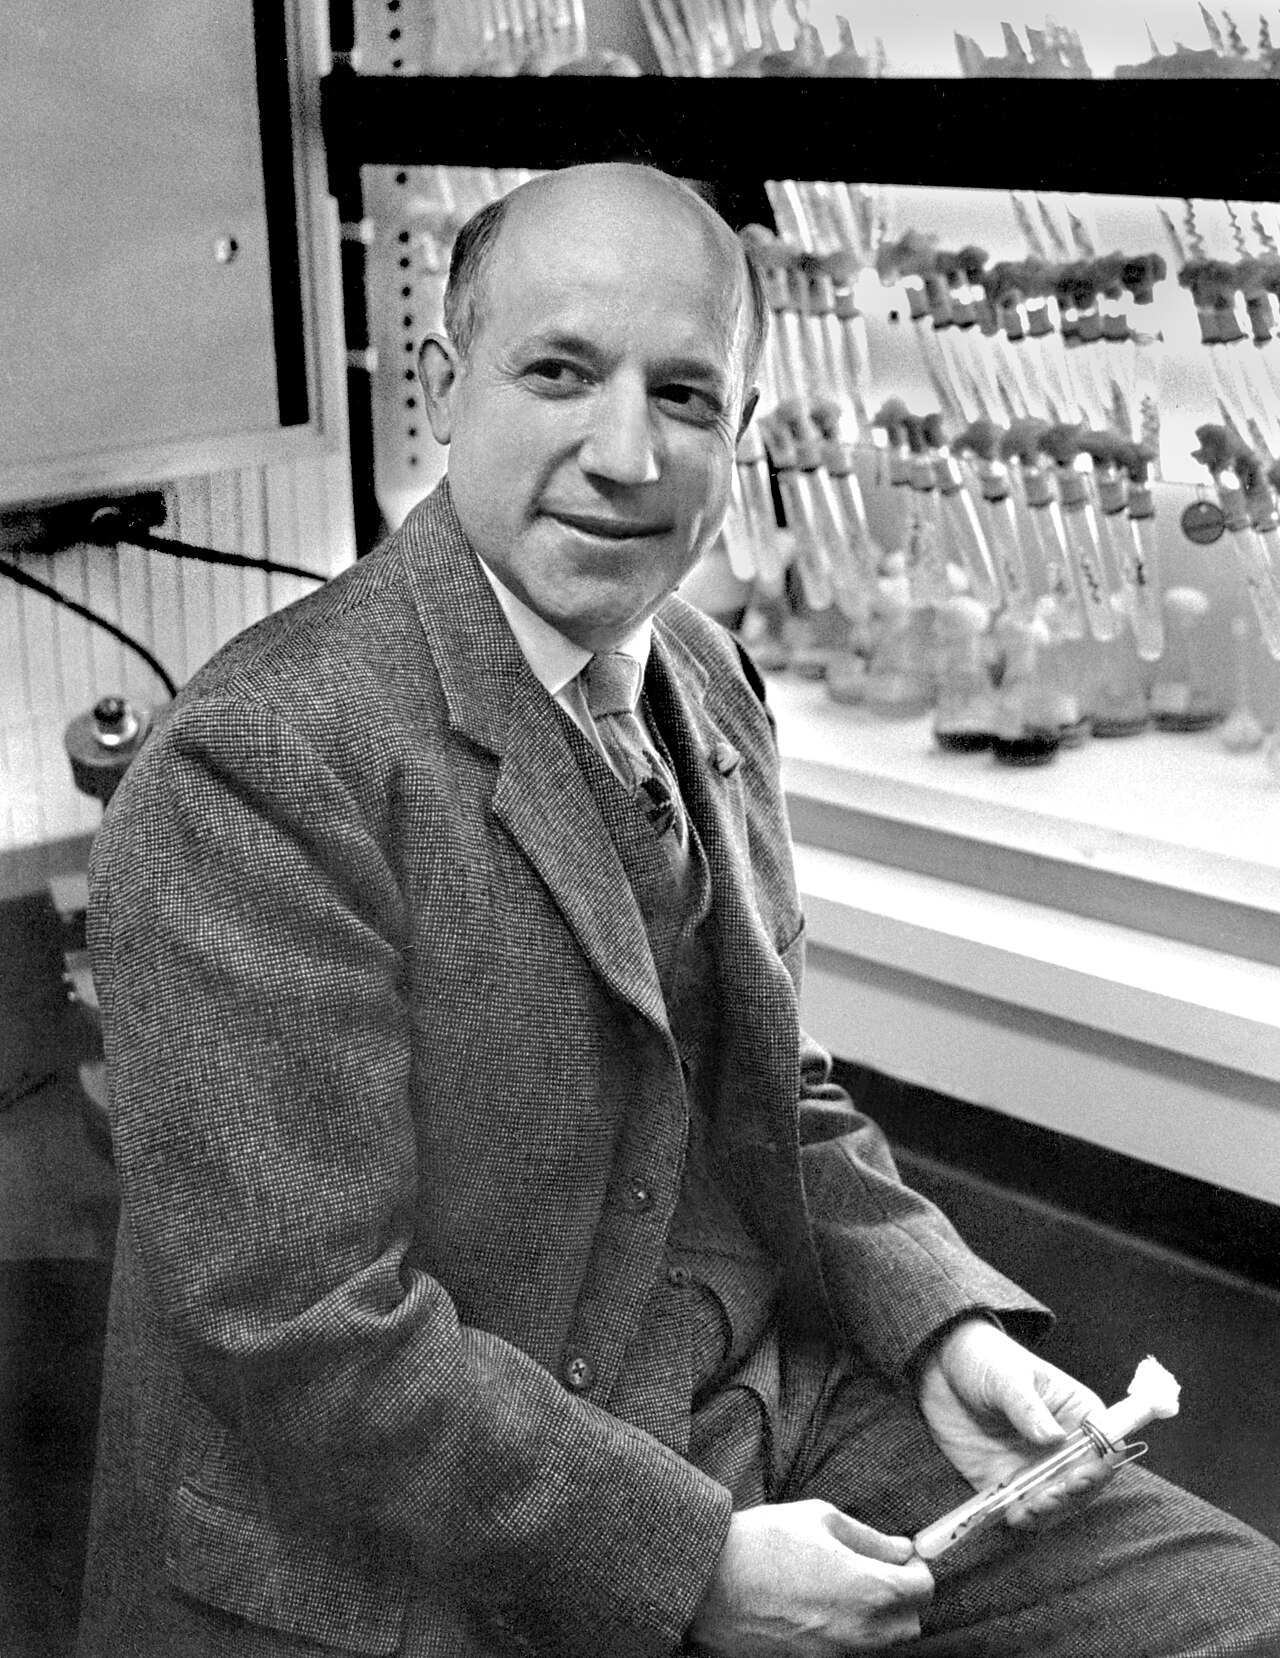
\includegraphics[width=0.26\linewidth]{images/book3/calvin.jpg}

{\small मेल्विन कैल्विन (1911--1997), जिन्होंने बेन्सन के साथ
रेडियोसक्रिय कार्बन और काग़ज़ वर्णलेखन से $\mathrm{CO_2}$ से शर्करा तक
कार्बन का पथ खोजा। छायाचित्र: लॉरेंस बर्कली प्रयोगशाला, सार्वजनिक
अधिकार-मुक्त।}
\end{omfigure}

\begin{omfigure}
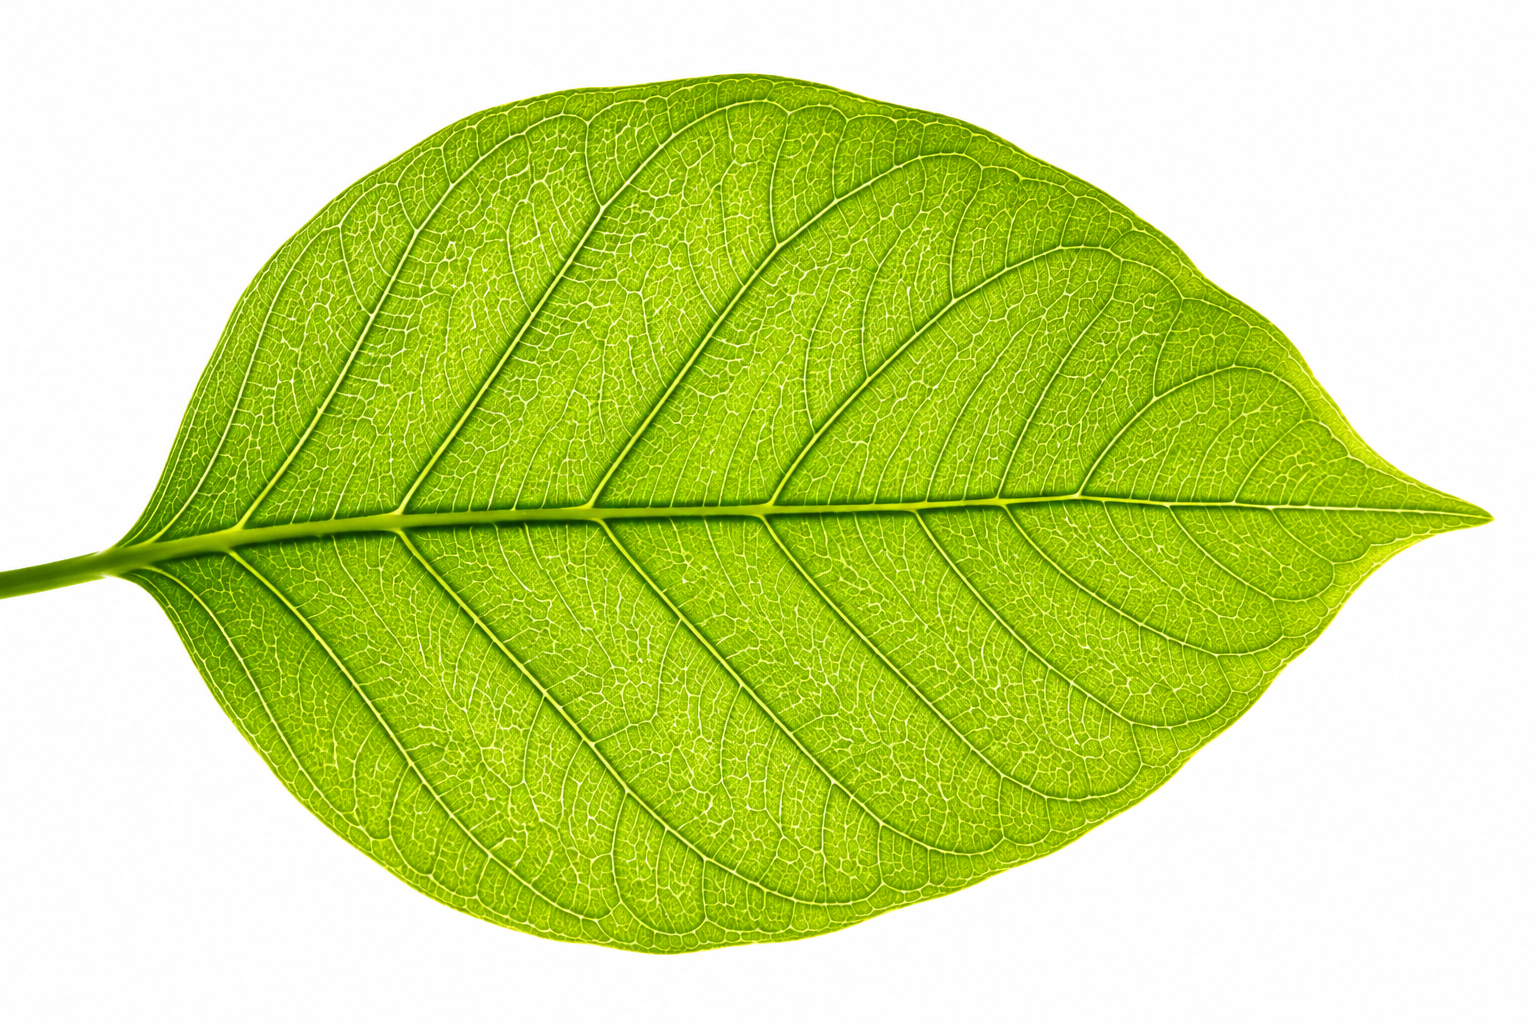
\includegraphics[width=0.6\linewidth]{images/book3/ai/b3-14-leaf-backlit.png}

{\small सूरज के सामने एक \omterm{def:b1:flowering-plant-organization:organs}{पत्ती}: जो प्रकाश वह अवशोषित करती है वह उसकी
खंभ \omterm{def:b1:cell-unit-of-life:cell}{कोशिकाओं} के हर \omterm{def:b1:photosynthesis:chloroplast}{हरितलवक} में जल का टूटना और उस कार्बन डाइऑक्साइड का
स्थिरीकरण चलाता है जो उसके \omterm{def:b1:flowering-plant-organization:tissues}{रंध्रों} से भीतर आई।}
\end{omfigure}

\begin{method}[किसी प्रकाश-संश्लेषी बजट का संतुलन]\label{met:b1:photosynthesis:budget}
\begin{enumerate}
  \item कार्बन गिनिए: स्थिर हुई हर $\mathrm{CO_2}$ उत्पाद का एक कार्बन
        देती है; एक ग्लूकोज़ को \omterm{def:b1:photosynthesis:fixation}{RuBisCO} के छह फेरे चाहिए।
  \item वाहक गिनिए: हर फेरे में 3 \omterm{def:b1:water-small-molecules:atp}{ATP} और 2 NADPH लगते हैं (प्रति G3P
        9 और 6); एक ग्लूकोज़ में 18 \omterm{def:b1:water-small-molecules:atp}{ATP} और 12 NADPH।
  \item फ़ोटॉन गिनिए: रैखिक प्रवाह प्रति $\mathrm{O_2}$ 2 NADPH और
        लगभग 3 \omterm{def:b1:water-small-molecules:atp}{ATP} देता है, 8 फ़ोटॉन के बदले (प्रति \omterm{def:b1:photosynthesis:zscheme}{प्रकाशतंत्र} 4); 12 NADPH
        को 6 $\mathrm{O_2}$ और 48 फ़ोटॉन चाहिए; और अतिरिक्त \omterm{def:b1:water-small-molecules:atp}{ATP}
        चक्रीय प्रवाह से आता है (कुछ और फ़ोटॉन)। प्रति
        $\mathrm{CO_2}$ लगभग 8 फ़ोटॉन: यही क्वांटम आवश्यकता है।
  \item ऊर्जा गिनिए: \qty{680}{nm} फ़ोटॉनों का एक मोल \qty{176}{kJ} है;
        48 फ़ोटॉन \qty{8450}{kJ} हैं, और ग्लूकोज़ में संचित
        \qty{2870}{kJ}: यानी अधिक से अधिक \qty{34}{\%}, इससे पहले कि
        परावर्तन, श्वसन और स्पेक्ट्रम के अनवशोषित भाग की कोई हानि गिनी
        जाए।
\end{enumerate}
\end{method}

\section{प्रकाश-श्वसन, C4 और CAM}

\begin{proposition}[RuBisCO का दोष]\label{prop:b1:photosynthesis:photorespiration}
\index{प्रकाश-श्वसन}
\omterm{def:b1:photosynthesis:fixation}{RuBisCO} $\mathrm{CO_2}$ की जगह $\mathrm{O_2}$ भी स्वीकार कर लेता है:
RuBP के ऑक्सीजनन से एक 3-PGA और एक दो-कार्बन फ़ॉस्फ़ोग्लाइकोलेट बनते हैं,
जिन्हें \omterm{def:b1:cell-unit-of-life:cell}{कोशिका} को तीन \omterm{def:b1:cell-unit-of-life:prokeuk}{कोशिकांगों} के आरपार एक महँगे रास्ते से बचाना पड़ता
है, जो $\mathrm{CO_2}$ छोड़ता है और \omterm{def:b1:water-small-molecules:atp}{ATP} खपाता है ---
यानी \emph{प्रकाश-श्वसन}। यह \omterm{def:b1:enzymes:enzyme}{एंजाइम} ठीक से भेद नहीं करता (बराबर
सांद्रताओं पर $\mathrm{CO_2}$ के पक्ष में लगभग \qty{80}{} बनाम 1),
और हवा में $\mathrm{O_2}$ $\mathrm{CO_2}$ से पाँच सौ गुना अधिक है;
\qty{25}{\celsius} पर एक-चौथाई स्थिरीकरण बरबाद जाते हैं, और गरम, सूखे
मौसम में उससे भी अधिक, जब रंध्र बंद हो जाते हैं और \omterm{def:b1:flowering-plant-organization:organs}{पत्ती} के भीतर
$\mathrm{CO_2}$ गिर जाती है। \omterm{def:b1:photosynthesis:fixation}{RuBisCO}, जो तब विकसित हुआ जब हवा में
ऑक्सीजन नहीं थी, धीमा भी है (प्रति सेकंड तीन चक्र) और उसकी भरपाई
प्रचुरता से होती है: वह पृथ्वी का सबसे बहुतायत वाला \omterm{def:b1:proteins:peptide}{प्रोटीन} है, और किसी
\omterm{def:b1:flowering-plant-organization:organs}{पत्ती} के घुलनशील \omterm{def:b1:proteins:peptide}{प्रोटीन} का आधा।
\end{proposition}

\begin{definition}[C4 और CAM पौधे]\label{def:b1:photosynthesis:c4cam}
\index{C4 पौधा}\index{CAM पौधा}
\emph{C4 पौधे} (मक्का, गन्ना, ज्वार, अनेक उष्णकटिबंधीय घासें)
$\mathrm{CO_2}$ गाढ़ी करके यह रिसाव सील कर देते हैं: मध्योतक \omterm{def:b1:cell-unit-of-life:cell}{कोशिकाओं} में
ऐसा \omterm{def:b1:enzymes:enzyme}{एंजाइम} (PEP कार्बोक्सिलेज़), जिसकी $\mathrm{O_2}$ से कोई बंधुता नहीं,
बाइकार्बोनेट को चार-कार्बन वाले किसी अम्ल में स्थिर करता है, जिसे शिराओं
के चारों ओर की \emph{पूल-आच्छद} \omterm{def:b1:cell-unit-of-life:cell}{कोशिकाओं} में भेजकर वहाँ विकार्बोक्सिलित
किया जाता है, जिससे \omterm{def:b1:photosynthesis:fixation}{RuBisCO} के चारों ओर $\mathrm{CO_2}$ दस गुना हो जाती
है और ऑक्सीजनन दब जाता है --- और इसकी क़ीमत प्रति $\mathrm{CO_2}$ दो
अतिरिक्त \omterm{def:b1:water-small-molecules:atp}{ATP} है। दोनों कोशिका-प्रकार मिलकर \emph{क्रांत्स} (``माला'')
शारीरिकी बनाते हैं। \emph{CAM पौधे}
(नागफनी, अनन्नास, रामबाँस) उन्हीं दोनों चरणों को स्थान के बजाय समय में
अलग करते हैं: वे अपने रंध्र रात में खोलते हैं, $\mathrm{CO_2}$ को
\omterm{def:b1:eukaryotic-cell:plantcell}{रसधानी} में मैलिक अम्ल के रूप में संचित करते हैं, और दिन में बंद \omterm{def:b1:flowering-plant-organization:tissues}{रंध्रों} के
पीछे उसे \omterm{def:b1:photosynthesis:fixation}{RuBisCO} को दे देते हैं, और प्रति स्थिर कार्बन किसी C3 पौधे से
दसवाँ भाग जल खोते हैं।
\end{definition}

\begin{omfigure}
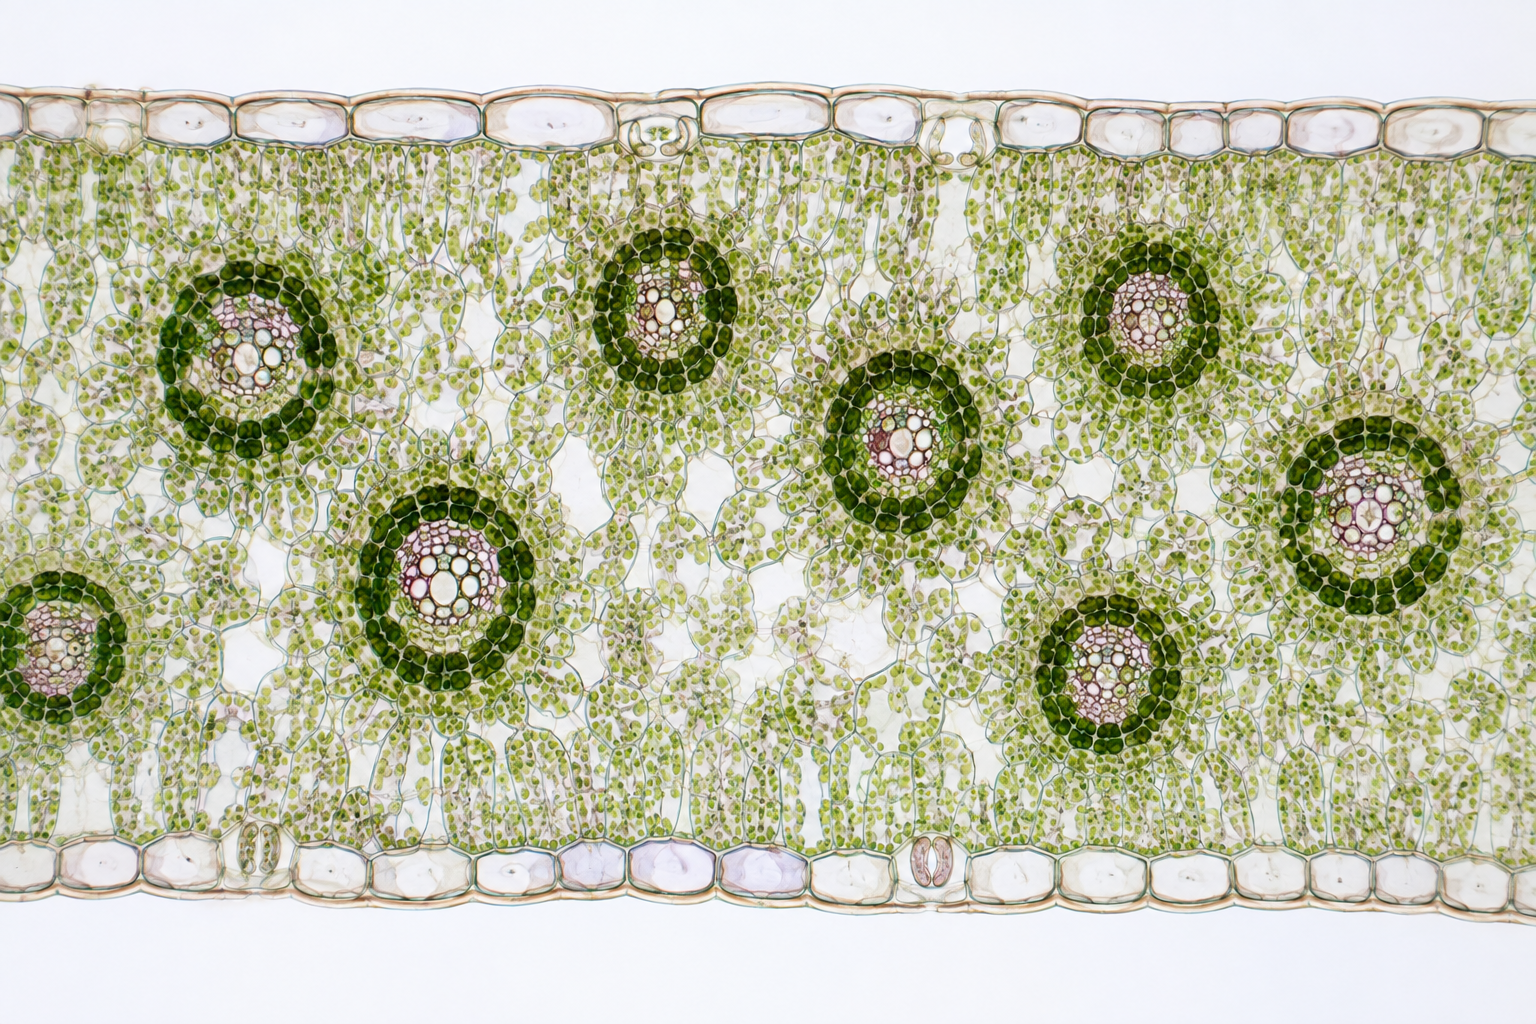
\includegraphics[width=0.6\linewidth]{images/book3/ai/b3-14-maize-kranz.png}

{\small मक्का की \omterm{def:b1:flowering-plant-organization:organs}{पत्ती} में क्रांत्स शारीरिकी: हर शिरा के चारों ओर
\omterm{def:b1:eukaryotic-cell:plastid}{हरितलवकों} से भरी बड़ी पूल-आच्छद \omterm{def:b1:cell-unit-of-life:cell}{कोशिकाओं} की माला है, और उसके चारों ओर
मध्योतक \omterm{def:b1:cell-unit-of-life:cell}{कोशिकाओं} का घेरा। $\mathrm{CO_2}$ बाहरी घेरे में पकड़ी जाती है
और भीतरी घेरे के \omterm{def:b1:photosynthesis:fixation}{RuBisCO} तक गाढ़ी होकर पहुँचाई जाती है।}
\end{omfigure}

\begin{example}[कौन-सा पौधा कहाँ]\label{ex:b1:photosynthesis:where}
नम हवा में \qty{20}{\celsius} पर किसी C3 गेहूँ की \omterm{def:b1:flowering-plant-organization:organs}{पत्ती} और किसी C4 मक्का
की \omterm{def:b1:flowering-plant-organization:organs}{पत्ती} लगभग एक ही दर से कार्बन स्थिर करती हैं, और मक्का प्रति कार्बन दो
\omterm{def:b1:water-small-molecules:atp}{ATP} अधिक चुकाता है। सूखी हवा में \qty{35}{\celsius} पर गेहूँ अपने
स्थिरीकरण का एक-तिहाई प्रकाश-श्वसन में खो देता है जबकि मक्का कुछ नहीं
खोता: C4 घासें गरम खुले देश पर छाई रहती हैं, और C3 पौधे ठंडे तथा छायादार
पर। कोई नागफनी दोनों मानकों से धीमे स्थिर करती है पर वहाँ जीवित रहती है
जहाँ बाक़ी प्यास से मर जाते।
\end{example}

\section{स्वपोषण}

\begin{definition}[स्वपोषण]\label{def:b1:photosynthesis:autotrophy}
कोई \omterm{def:b1:organism-environment:organism}{जीव} तब \emph{स्वपोषी}\index{स्वपोषण} है जब वह अपना कार्बनिक पदार्थ
$\mathrm{CO_2}$ से बनाता हो (\cref{ch:b1:organism-environment})।
उसे एक ऊर्जा-स्रोत और एक इलेक्ट्रॉन-स्रोत चाहिए।
\emph{\omterm{def:b1:organism-environment:trophy}{प्रकाशस्वपोषी}} ऊर्जा प्रकाश से लेते हैं: पौधे, शैवाल और
सायनोबैक्टीरिया अपने इलेक्ट्रॉन जल से लेते हैं और ऑक्सीजन छोड़ते हैं
(\emph{ऑक्सीजनी}); बैंगनी और हरे जीवाणु उन्हें हाइड्रोजन
सल्फ़ाइड या कार्बनिक अम्लों से लेते हैं और कुछ नहीं छोड़ते।
\emph{\omterm{def:b1:organism-environment:trophy}{रसायनस्वपोषी}} ऊर्जा और इलेक्ट्रॉन दोनों अकार्बनिक यौगिकों के
ऑक्सीकरण से लेते हैं --- अमोनिया, नाइट्राइट, सल्फ़ाइड, हाइड्रोजन,
फ़ेरस लोहा --- और बिना किसी प्रकाश के: मिट्टी के नाइट्रीकारी जीवाणु, और
वे जीवाणु जो गहरे समुद्री छिद्रों के पारितंत्र खिलाते हैं। सभी कार्बन
स्थिर करने के लिए \omterm{def:b1:photosynthesis:fixation}{कैल्विन चक्र}, या उससे जुड़ा कोई चक्र, काम में लेते हैं;
सभी उसे NADPH से अपचयित करते हैं और \omterm{def:b1:water-small-molecules:atp}{ATP} से क़ीमत चुकाते हैं; और वे केवल
इसमें भिन्न हैं कि \omterm{def:b1:water-small-molecules:atp}{ATP} तथा इलेक्ट्रॉन कहाँ से आते हैं।
\end{definition}

\begin{example}[वैश्विक बजट]\label{ex:b1:photosynthesis:global}
प्रकाश-संश्लेषण हर वर्ष ज़मीन पर लगभग \qty{120}{Gt} कार्बन स्थिर करता है
और महासागरों में \qty{50}{Gt}, जिसका आधा एककोशिकीय शैवाल तथा
सायनोबैक्टीरिया करते हैं जो आँख से दिखते ही नहीं; वह वायुमंडल की कार्बन
डाइऑक्साइड हर सात वर्ष में और उसकी ऑक्सीजन हर दो हज़ार वर्ष में पलट देता
है। ऑक्सीजन भी उसी रास्ते आई: दो अरब वर्ष तक सायनोबैक्टीरिया उसे ऐसे
वायुमंडल में छोड़ते रहे जिसमें वह थी ही नहीं, और हर वायुजीवी \omterm{def:b1:organism-environment:organism}{जीव},
\omterm{def:b1:eukaryotic-cell:mitochondrion}{सूत्रकणिका} से लेकर ऊपर तक, उसी एक \omterm{def:b1:enzymes:enzyme}{एंजाइम} तंत्र के रिसाव पर बना है जो जल
तोड़ता है।
\end{example}

\section{अभ्यास}

\begin{exercise}[$\star$]\label{exo:b1:photosynthesis:1}
\omterm{def:b1:photosynthesis:chloroplast}{हरितलवक} के तीनों झिल्ली तंत्र बताइए और यह भी कि \omterm{prop:b1:photosynthesis:lightreactions}{प्रकाश अभिक्रियाएँ} तथा
\omterm{def:b1:photosynthesis:fixation}{कैल्विन चक्र} कहाँ होते हैं।
\end{exercise}

\begin{exercise}[$\star$]\label{exo:b1:photosynthesis:2}
प्रकाश अभिक्रियाओं का समीकरण लिखिए और बताइए कि छूटी हुई ऑक्सीजन कहाँ से
आती है, साक्ष्य सहित।
\end{exercise}

\begin{exercise}[$\star$]\label{exo:b1:photosynthesis:3}
\omterm{def:b1:photosynthesis:fixation}{कैल्विन चक्र} के तीनों चरण बताइए और प्रति स्थिर $\mathrm{CO_2}$ खपे \omterm{def:b1:water-small-molecules:atp}{ATP}
तथा NADPH की संख्या।
\end{exercise}

\begin{exercise}[$\star$]\label{exo:b1:photosynthesis:4}
स्पेक्ट्रम वाले आलेख से बताइए कि \omterm{def:b1:photosynthesis:pigments}{पर्णहरित} $a$ किन तरंगदैर्घ्यों पर सबसे
अधिक अवशोषित करता है, और \qty{500}{nm} के आसपास क्रिया स्पेक्ट्रम
\omterm{def:b1:photosynthesis:pigments}{पर्णहरित} के अवशोषण से ऊँचा क्यों है।
\end{exercise}

\begin{exercise}[$\star\star$]\label{exo:b1:photosynthesis:5}
एमरसन का संवर्धन प्रभाव समझाइए और यह भी कि उसने प्रकाश अभिक्रियाओं के
संगठन के बारे में क्या दिखाया।
\end{exercise}

\begin{exercise}[$\star\star$]\label{exo:b1:photosynthesis:6}
\qty{0.18}{V} का कोई प्रोटॉन-प्रेरक बल प्रति मोल प्रोटॉन कितनी \omterm{prop:b1:water-small-molecules:gibbs}{मुक्त
ऊर्जा} के बराबर है ($F = \qty{96500}{C/mol}$)? \qty{50}{kJ/mol} पर एक \omterm{def:b1:water-small-molecules:atp}{ATP}
बनाने के लिए कितने प्रोटॉन बहने चाहिए? सिंथेज़ जिन चार को काम में लेता है
उनसे तुलना कीजिए।
\end{exercise}

\begin{exercise}[$\star\star$]\label{exo:b1:photosynthesis:7}
यागेनडॉर्फ़ के थाइलेकॉइडों ने अम्ल-स्नान के बाद अँधेरे में \omterm{def:b1:water-small-molecules:atp}{ATP} बनाया।
समझाइए कि इससे क्या सिद्ध होता है और क्या नहीं, और भविष्यवाणी कीजिए कि
स्थानांतरण से पहले कोई अयुग्मक मिला दिया जाए तो परिणाम क्या होगा।
\end{exercise}

\begin{exercise}[$\star\star$]\label{exo:b1:photosynthesis:8}
कार्बन का पीछा कीजिए: 3 RuBP (15 कार्बन) और 3
$\mathrm{CO_2}$ से शुरू करके 3-PGA, G3P, निर्यात हुए G3P और
पुनर्जनित RuBP तक कार्बन गिनिए, और संतुलन जाँचिए।
\end{exercise}

\begin{exercise}[$\star\star$]\label{exo:b1:photosynthesis:9}
कैल्विन के प्रयोग में $\mathrm{CO_2}$ हटाने पर RuBP बढ़ता है और 3-PGA
गिरता है; प्रकाश बंद करने पर 3-PGA बढ़ता है और RuBP गिरता है।
चक्र से दोनों समझाइए।
\end{exercise}

\begin{exercise}[$\star\star\star$]\label{exo:b1:photosynthesis:10}
\qty{680}{nm} फ़ोटॉनों के एक मोल की ऊर्जा निकालिए ($h =
\qty{6.63e-34}{J.s}$, $c = \qty{3.0e8}{m/s}$, $N_A = \num{6.02e23}$),
प्रति ग्लूकोज़ चाहिए 48 फ़ोटॉनों की ऊर्जा, और \qty{2870}{kJ/mol} संचित
करने की दक्षता। किसी पूरी फ़सल की दक्षता, जो धूप का लगभग \qty{1}{\%} है,
इतनी कम क्यों है?
\end{exercise}

\begin{exercise}[$\star\star\star$]\label{exo:b1:photosynthesis:11}
हवा में \qty{25}{\celsius} पर \omterm{def:b1:photosynthesis:fixation}{RuBisCO} हर तीन कार्बोक्सिलनों पर एक बार
ऑक्सीजनन करता है; और हर ऑक्सीजनन बचाव में आधी $\mathrm{CO_2}$ छोड़ता है
तथा \omterm{def:b1:water-small-molecules:atp}{ATP} ख़र्च करता है। प्रति 100
कार्बोक्सिलन शुद्ध स्थिर कार्बन और खोया भिन्न निकालिए। कोई \omterm{def:b1:photosynthesis:c4cam}{C4 पौधा} यह
हानि टाल देता है पर प्रति $\mathrm{CO_2}$ 2 अतिरिक्त \omterm{def:b1:water-small-molecules:atp}{ATP} ख़र्च करता है:
यदि एक \omterm{def:b1:water-small-molecules:atp}{ATP} लगभग एक स्थिर $\mathrm{CO_2}$ के दसवें भाग जितना हो, तो
हानि के किस भिन्न पर C4 अभिकल्पना फ़ायदेमंद हो जाती है?
\end{exercise}

\begin{exercise}[$\star\star\star$]\label{exo:b1:photosynthesis:12}
``प्रकाश-संश्लेषण उल्टा चलाया गया श्वसन है।'' एक अनुच्छेद में चर्चा कीजिए,
और रसोपरासरणी क्रियाविधि, इलेक्ट्रॉन प्रवाह की दिशा, वाहकों और चक्रों की
तुलना करते हुए बताइए कि यह उपमा कहाँ टिकती है और कहाँ चूक जाती है।
\end{exercise}

\section{समस्या: ग्लूकोज़ के एक अणु की क़ीमत}

\begin{problem}[{सप्ताहांत समस्या --- फ़ोटॉन गिने गए, थाइलेकॉइड के
आरपार इलेक्ट्रॉनों तथा प्रोटॉनों का पीछा किया गया, ATP और NADPH आँके तथा
ख़र्च किए गए, किसी पत्ती की दैनिक फ़सल तौली गई, और अंत में
प्रकाश-संश्लेषण की ऊर्जा-दक्षता}]
\label{pb:b1:photosynthesis:1}
स्थिरांक: $h = \qty{6.63e-34}{J.s}$, $c = \qty{3.00e8}{m/s}$,
$N_A = \num{6.02e23}$, $F = \qty{96500}{C/mol}$, $R = \qty{8.314}{J.mol^{-1}.K^{-1}}$,
$T = \qty{298}{K}$। ग्लूकोज़ के दहन की \omterm{prop:b1:water-small-molecules:gibbs}{मुक्त ऊर्जा}
\qty{2870}{kJ/mol}; \omterm{def:b1:photosynthesis:chloroplast}{हरितलवक} में \omterm{def:b1:water-small-molecules:atp}{ATP} संश्लेषण की क़ीमत
\qty{50}{kJ/mol}; NADPH \qty{220}{kJ/mol} अपचायक शक्ति रखता है।

\medskip
\noindent\textbf{भाग I --- फ़ोटॉन और इलेक्ट्रॉन।}
\begin{enumerate}
  \item \qty{680}{nm} के एक फ़ोटॉन की और उनके एक मोल की ऊर्जा
        निकालिए।
  \item \qty{700}{nm} फ़ोटॉनों के एक मोल की और \qty{450}{nm}
        फ़ोटॉनों के एक मोल की ऊर्जा निकालिए। नीला प्रकाश प्रति फ़ोटॉन
        लाल से अधिक प्रकाश-संश्लेषण क्यों नहीं देता?
  \item \qty{680}{nm} के कितने फ़ोटॉन एक जूल ढोते हैं?
  \item एक इलेक्ट्रॉन को जल ($E'_0 = \qty{+0.82}{V}$) से
        $\mathrm{NADP^+}$ ($E'_0 = \qty{-0.32}{V}$) तक ले जाने में प्रति
        मोल इलेक्ट्रॉन कितनी \omterm{prop:b1:water-small-molecules:gibbs}{मुक्त ऊर्जा} चाहिए ($\Delta G = -nF\Delta E$)?
  \item प्रति इलेक्ट्रॉन दो फ़ोटॉन काम में आते हैं (हर \omterm{def:b1:photosynthesis:zscheme}{प्रकाशतंत्र} में एक)।
        प्रति मोल इलेक्ट्रॉन दी गई ऊर्जा और उसका वह भिन्न निकालिए जो
        अपचयोपचय परिवर्तन में संचित होता है।
  \item एक $\mathrm{O_2}$ और दो NADPH बनाने के लिए कितने इलेक्ट्रॉन,
        और इस तरह कितने फ़ोटॉन चाहिए?
  \item यदि 12 NADPH चाहिए तो प्रति ग्लूकोज़ कितने फ़ोटॉन?
\end{enumerate}

\medskip
\noindent\textbf{भाग II --- प्रोटॉन और \omterm{def:b1:water-small-molecules:atp}{ATP}।}
छूटी हुई हर $\mathrm{O_2}$ के लिए जल के टूटने से अवकाशिका में चार
प्रोटॉन मुक्त होते हैं और साइटोक्रोम $b_6f$ संकुल आठ पंप करता है;
और \omterm{thm:b1:photosynthesis:chemiosmosis}{ATP सिंथेज़} प्रति \omterm{def:b1:water-small-molecules:atp}{ATP} \qty{4}{H^+} काम में लेता है। अवकाशिका
pH 5 पर है और \omterm{def:b1:photosynthesis:chloroplast}{पीठिका} pH 8 पर; \omterm{def:b1:photosynthesis:chloroplast}{थाइलेकॉइड} के आरपार \omterm{def:b1:membranes-transport:potential}{झिल्ली विभव}
नगण्य है।
\begin{enumerate}[resume]
  \item pH के अंतर से प्रोटॉन-प्रेरक बल वोल्ट में निकालिए
        ($\Delta\mu = 2.303\,RT\,\Delta\mathrm{pH}/F$), और प्रति मोल
        प्रोटॉन \omterm{prop:b1:water-small-molecules:gibbs}{मुक्त ऊर्जा} भी।
  \item प्रति $\mathrm{O_2}$ अवकाशिका में पहुँचाए गए प्रोटॉन और उनसे बन
        सकने वाला \omterm{def:b1:water-small-molecules:atp}{ATP} निकालिए।
  \item रैखिक प्रवाह से प्रति ग्लूकोज़ (6
        $\mathrm{O_2}$) बना \omterm{def:b1:water-small-molecules:atp}{ATP} निकालिए, और \omterm{def:b1:photosynthesis:fixation}{कैल्विन चक्र} को चाहिए 18
        से तुलना कीजिए। कमी कैसे पूरी होती है?
  \item प्रति \omterm{def:b1:water-small-molecules:atp}{ATP} (\qty{4}{H^+}) प्रोटॉनों से उपलब्ध \omterm{prop:b1:water-small-molecules:gibbs}{मुक्त ऊर्जा} और
        सिंथेज़ की दक्षता निकालिए।
  \item किसी \omterm{def:b1:photosynthesis:chloroplast}{हरितलवक} की अवकाशिका का आयतन लगभग
        \qty{1}{\micro m^3} है। pH 5 पर वह कितने मुक्त प्रोटॉन रखती
        है? इसकी तुलना उन मोटे तौर पर $10^5$ प्रोटॉनों से कीजिए जो हर
        सेकंड सिंथेज़ों से होकर जाते हैं, और निष्कर्ष निकालिए कि
        अवकाशिका को क्या \omterm{def:b1:water-small-molecules:buffer}{बफ़र} करता है।
\end{enumerate}

\medskip
\noindent\textbf{भाग III --- शर्करा।}
\begin{enumerate}[resume]
  \item प्रति ग्लूकोज़ संचित ऊर्जा 18 \omterm{def:b1:water-small-molecules:atp}{ATP} $\times$
        \qty{50}{kJ} और 12 NADPH $\times$ \qty{220}{kJ} के योग के रूप
        में लिखिए, और उसकी तुलना ग्लूकोज़ के \qty{2870}{kJ} से कीजिए।
        अंतर कहाँ जाता है?
  \item प्रश्न 6 के 48 फ़ोटॉनों की ऊर्जा और फ़ोटॉन से ग्लूकोज़ तक
        प्रकाश-संश्लेषण की दक्षता निकालिए।
  \item धूप का केवल \qty{45}{\%} उन तरंगदैर्घ्यों में है जिन्हें वर्णक
        अवशोषित करते हैं, और उसका दसवाँ भाग परावर्तित या पारगमित हो
        जाता है। आपाती धूप से ग्लूकोज़ तक की दक्षता निकालिए, श्वसन से
        पहले।
  \item \qty{50}{cm^2} की कोई \omterm{def:b1:flowering-plant-organization:organs}{पत्ती} \qty{10}{h} तक \qty{400}{W/m^2}
        धूप पाती है। मिली ऊर्जा और, प्रश्न 14 की दक्षता पर, बनी
        ग्लूकोज़ ग्राम में निकालिए (\qty{180}{g/mol})।
  \item \omterm{def:b1:flowering-plant-organization:organs}{पत्ती} जीवित रहने के लिए उस ग्लूकोज़ का \qty{40}{\%} श्वसन में
        जला देती है। उसका शुद्ध लाभ ग्लूकोज़ के ग्राम में और कार्बन के
        ग्राम में क्या है?
  \item कोई फ़सल एक ऋतु में कुल \qty{1}{\%} दक्षता तक पहुँचती है।
        जो पहले ही गिनी जा चुकीं उनसे परे तीन ऐसी हानियाँ गिनाइए जो
        \omterm{def:b1:flowering-plant-organization:organs}{पत्ती} के आँकड़े को फ़सल के आँकड़े से अलग करती हैं।
\end{enumerate}

\medskip
\noindent\textbf{भाग IV --- रिसाव।}
हवा में \qty{25}{\celsius} पर \omterm{def:b1:photosynthesis:fixation}{RuBisCO} हर तीन कार्बोक्सिलनों पर एक
ऑक्सीजनन करता है; और हर ऑक्सीजनन की क़ीमत आधी स्थिर
$\mathrm{CO_2}$ तथा 3.5 \omterm{def:b1:water-small-molecules:atp}{ATP} के बराबर है।
\begin{enumerate}[resume]
  \item प्रति 100 कार्बोक्सिलन ऑक्सीजनन, खोया कार्बन और कमाया गया
        शुद्ध कार्बन निकालिए।
  \item प्रति 100 कार्बोक्सिलन बचाव पर ख़र्च \omterm{def:b1:water-small-molecules:atp}{ATP} और प्रति शुद्ध कमाए
        कार्बन कुल \omterm{def:b1:water-small-molecules:atp}{ATP} निकालिए (प्रति कार्बोक्सिलन \omterm{def:b1:photosynthesis:fixation}{कैल्विन चक्र} के 3
        \omterm{def:b1:water-small-molecules:atp}{ATP} और बचाव मिलाकर)।
  \item किसी C4 पौधे में कोई ऑक्सीजनन नहीं होता पर वह प्रति पहुँचाई गई
        $\mathrm{CO_2}$ 2 अतिरिक्त \omterm{def:b1:water-small-molecules:atp}{ATP} ख़र्च करता है। उसका प्रति शुद्ध
        कार्बन \omterm{def:b1:water-small-molecules:atp}{ATP} निकालिए और तुलना कीजिए।
  \item \qty{35}{\celsius} पर ऑक्सीजनन का अनुपात बढ़कर दो में एक हो
        जाता है। C3 के आँकड़े फिर से निकालिए और बताइए कि कौन-सी
        अभिकल्पना जीतती है।
  \item समझाइए कि किसी हरितगृह की $\mathrm{CO_2}$ वायुमंडलीय मान की
        तिगुनी करने से C3 फ़सलों (टमाटर, गेहूँ) की उपज क्यों बढ़ती है
        पर C4 फ़सलों (मक्का) की मुश्किल से।
  \item कोई C3 \omterm{def:b1:flowering-plant-organization:organs}{पत्ती} प्रति स्थिर $\mathrm{CO_2}$ लगभग 250 जल-अणु खोती
        है, और कोई \omterm{def:b1:photosynthesis:c4cam}{CAM पौधा} लगभग 25। \qty{1}{g} कार्बन स्थिर करने के
        लिए हर एक कितना जल खोता है, यह निकालिए।
  \item परिणाम बताइए: प्रति $\mathrm{CO_2}$ क्वांटम आवश्यकता,
        फ़ोटॉन से ग्लूकोज़ तक की दक्षता, और धूप से \omterm{def:b1:flowering-plant-organization:organs}{पत्ती} की शुद्ध
        शर्करा तक की दक्षता।
\end{enumerate}
\end{problem}
